\begin{figure}[h!]
    \centering
    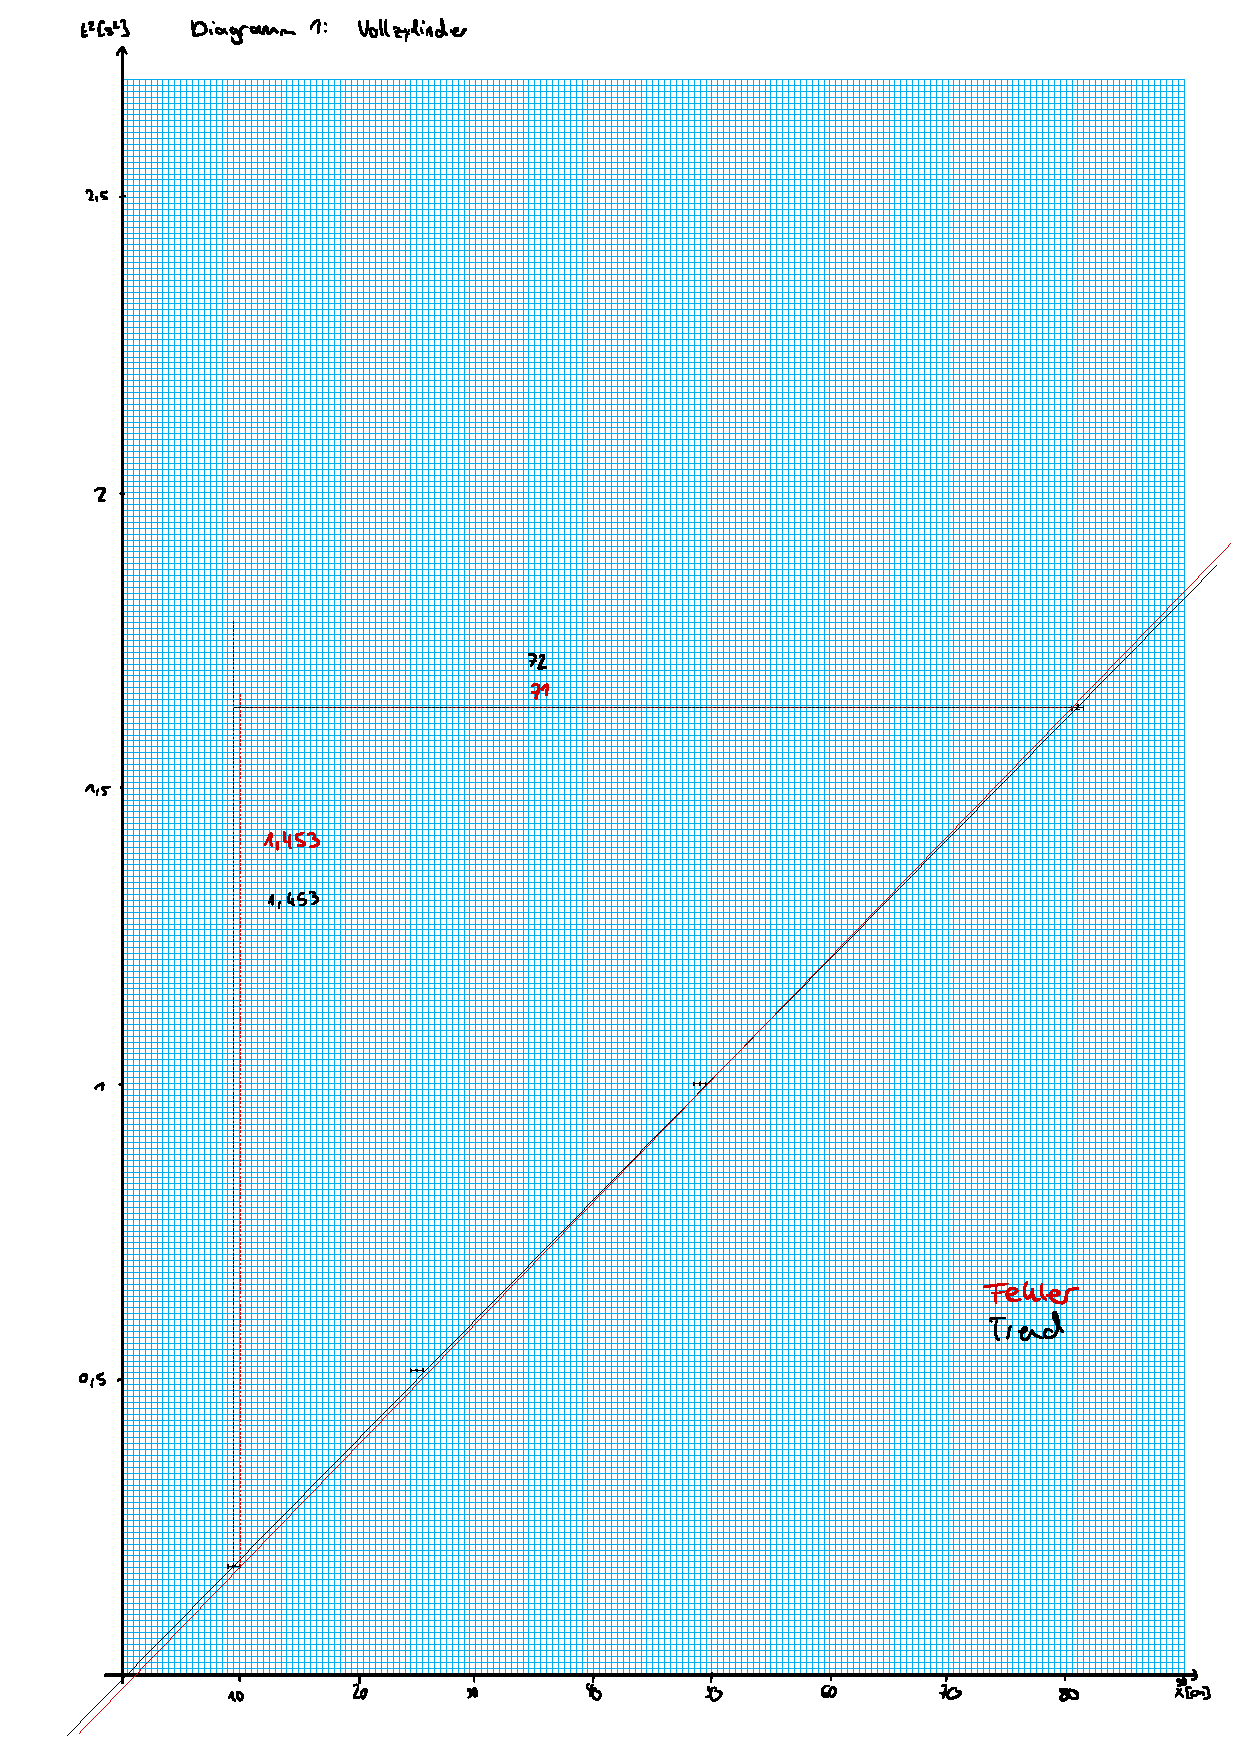
\includegraphics[page=1, width=.95\textwidth,]{Diagramme15.pdf}
    \caption{Diagramm 1}
\end{figure}
\newpage
\begin{figure}[h!]
    \centering
    \includegraphics[page=2, width=1\textwidth,]{Diagramme15.pdf}
    \caption{Diagramm 2}
\end{figure}
\newpage



\section{Aufgabe I}
\subsection{Vollzylinder}

Zuerst wird die theoretische Beschleunigung des Vollzylinders berechnet, dafür benötigt man das Trägheitsmoment
um die Rotationsachse, dabei gilt für die Dichte $\rho_{Al} = \SI{2,70}{\frac{\gram}{\cm^3}}$.
Mit der Masse $m_V = \SI{444 \pm 1}{\gram}$ und dem Radius $r = \SI{2,5000\pm 0,0025}{\cm}$ ergibt sich nach Gleichung \ref{eq:JVoll} für das Trägheitsmoment:

\[ J_V = \SI{1,388 \pm 0,004}{\cdot 10^{-4} \kilogram \cdot \meter^2} \]

Der Fehler für $J_V$ wird berechnet durch:
\begin{equation}
    \Delta J_V = \frac{1}{2}\sqrt{(r^2 \Delta m)^2 + (2mr\Delta r)^2}
\end{equation}

Damit lässt sich aus Gleichung \ref{eq:a} die Beschleunigung des Körpers berechnen:

\[\boxed{a_V = \SI{1,06 \pm 0,03}{\frac{\meter}{\second^2}}}\]

Dabei gilt für den Fehler:

\begin{equation}
    \Delta a=\sqrt{\frac{J^{2} \Delta m^{2}}{m^{2} \left(J + m r^{2}\right)^{2}} + \frac{4 J^{2} \Delta r^{2}}{r^{2} \left(J + m r^{2}\right)^{2}} + \frac{\Delta J^{2}}{\left(J + m r^{2}\right)^{2}} + \frac{\Delta h^{2}}{h^{2}} + \frac{\Delta l^{2}}{l^{2}}}\cdot a
\end{equation}

\subsection{Hohlzylinder}

Die Rechnung erfolgt analog für den Holzylinder aus Messing. Dafür wird hier Gleichung \ref{eq: JHohl} verwendet.
Als Masse gilt $m=\SI{442 \pm 1}{\gram}$ und für die Radien $r_2 = \SI{2,5025 \pm 0,0025}{\cm}$, $r_1 = \SI{2,0350\pm 0,0025}{\cm}$.

\[ J_H = \SI{2,299 \pm 0,006}{\cdot 10^{-4} \kilogram \cdot \meter^2}\]

Für den Fehler gilt:
\begin{equation}
    \Delta J_H=\sqrt{\frac{1}{4} \Delta m^{2} \left(r_{1}^{2} + r_{2}^{2}\right)^{2} + \Delta r_{1}^{2} m^{2} r_{1}^{2} + \Delta r_{2}^{2} m^{2} r_{2}^{2}}
\end{equation}

Daraus kann erneut die Beschleunigung mit Gleichung \ref{eq:a} berechnet werden:

\[\boxed{a_V =  \SI{0,86 \pm 0,03}{\frac{\meter}{\second^2}}}\]


\subsection{Auswertung der Messwerte}

\begin{table}[h!]
    \centering
    \begin{tabular}{c c c c c}
        \toprule
        Zylinder & Schranke 1 $\overline{t_1}$[s] & Schranke 2 $\overline{t_2}$[s] & Schranke 3 $\overline{t_3}$[s] & Schranke 4 $\overline{t_4}$[s] \\
        \midrule
        Vollzylinder & $0,4280 \pm 0,0010 $ & $ 0,7182 \pm 0.0011$ & $0,9984 \pm 0,0011 $ & $ 1,2798 \pm 0,0011$\\
        Hohlzylinder & $0,471 \pm 0.004$ & $0,794 \pm 0,004$ & $1,1088 \pm 0,0024$ & $1,423 \pm 0,004$\\
        \bottomrule
    \end{tabular}
    \caption{Mittelwerte der Zeitmessungen}
\end{table}

Der Fehler wurde brechnet mithilfe des statistischen Fehlers $\sigma_{stat}$ und dem systematischen Fehler $\Delta t_{sys}$:
\begin{equation}
    \Delta t = \sqrt{(\sigma_{stat})^2 + (\Delta t_{sys})^2}
    \label{eq:FehlerTab}
\end{equation}

\subsection{Bestimmung von $a$ durch die Messung}

\subsubsection{Vollzylinder}

Für die Fehlerbalken in Diagramm 1 gilt folgende Formel:
\begin{equation}
    \Delta (t^2) = 2t\Delta t
\end{equation}

Aus dem Diagramm lässt sich die Steigung der Tredgeraden ermitteln.
Aus:
\begin{equation}
    s = \frac{1}{2} at^2
\end{equation}
Folgt, dass die Steigung genau $\frac{2}{a}$ entsprechen muss.
Für die Steigung gilt:

\[\varsigma = \SI{2.018 \pm 0,029}{\frac{\second^2}{\meter}} \]
Der Fehler ist heir die Differenz der Steigung zu Steigung der Fehlergeraden.
Aus $m$ lässt sich dann $a$ berechnen als:
\[\boxed{a = \SI{ 0,9910 \pm 0,014 }{\frac{\meter}{\second^2}}}\]
Der Fehler wird berechnet durch:
\begin{equation}
    \Delta a = \frac{2}{m^2}\Delta m
\end{equation}


\subsubsection{Hohlzylinder}

Dieselben Überlegungen gelten für den Hohlzylinder. Die Werte wurden in Diagramm 2 aufgetragen.

Für die Steigung gilt:

\[\varsigma = \SI{2.50 \pm 0,04}{\frac{\second^2}{\meter}} \]

Daraus folgt für die Beschleunigung:
\[\boxed{a = \SI{ 0,800 \pm 0,013}{\frac{\meter}{\second^2}}}\]

\newpage
\section{Aufgabe II}

\subsection{Vollzylinder}

\subsubsection{Translationsenergie}
Um die translations Energie zu bestimmmen wird die mittlere Zeit $t_m$zwischen den Lichtschranken an der Ebene nach der schiefen Ebene bestimmt. Dabei gilt der Fehler:
\begin{equation}
    \Delta t_m = \sqrt{(\Delta t_1)^2+ (\Delta t_2)^2}
\end{equation}
Anschließend wird das Mittel dieser Zeiten bestimmt, mit dem Fehler nach Gleichung \ref{eq:FehlerTab}.

\[\overline{t_{trans}} = \SI{0,2358 \pm 0,0011}{\second}\]

Der Abstand zwischen beiden Lichtschranken beträgt $s = \SI{30,0 \pm 0,5}{\cm}$. Daraus ergibt sich nach Gleichung \ref{eq:ETrans}:

\[E_{trans,voll} = \SI{0,359\pm 0,013}{\joule}\]

Der Fehler berechnet sich durch:

\begin{equation}
    \Delta E_{trans} = \frac{1}{2}\sqrt{\left(\left(\frac{s}{t_{trans}}\right)^2\Delta m\right)^2 + \left(\frac{2sm}{(t_{trans})^2}\Delta s\right)^2 +\left(2\left(\frac{s^2}{(t_{trans})^3}\right)\Delta t_{trans}\right)^2}
\end{equation}

\subsubsection{Rotationsenergie}

Für die Rotationsenergie gilt nach Gleichung \ref{eq:ERot}:

\[E_{rot,voll} = \SI{0,179 \pm 0,007}{\joule}\]

Für den Fehler gilt hier:
\[\Delta E_{rot}=\sqrt{\frac{s^{2} \left[J^{2} \Delta r^{2} s^{2} (t_{trans})^{2} + J^{2} \Delta (t_{trans})^{2} r^{2} s^{2} + r^{2} (t_{trans})^{2} \left(J^{2} \Delta s^{2} + 0.25 \Delta J^{2} s^{2}\right)\right]}{r^{6} (t_{trans})^{6}}}\]
Um auf die gesamte kinetische Energie zu kommen werden beide Energien addiert
\[\Rightarrow \boxed{E_{kin, voll} = \SI{0,538 \pm 0,015}{\joule}}\]

Für den Fehler gilt hier:
\begin{equation}
    \Delta E_{kin} = \sqrt{(\Delta E_{trans})^2 + (\Delta E_{rot})^2 }
\end{equation}

\subsubsection{Potentielle Energie}

Für die potentielle Energie wird die Auflagehöhe des Zylinders benötigt. Da unten an der schiefen Ebene ebenfalls eine Platte gleicher Bauart angebracht war,
wurde der relative Abstand dieser zum Auflagepunkt des Zylinders auf $h_s = \SI{14,2 \pm 1,0}{\cm}$ gemessen.
Um auf die Höhe des Schwerpunkts zu kommen muss nun noch der Radius des Vollzylinders addiert werden.
Damit gilt für die Höhe des Schwerpunkts:
\[h_{SP} = \SI{16,7 \pm 1,0}{\cm}\]
Dabei gilt für den Fehler:
\begin{equation}
    \Delta h_{SP} = \sqrt{(\Delta r)^2 + (\Delta h)^2}
\end{equation}
Damit gilt nach Gleichnung \ref{eq:pot}:
\[\boxed{E_{pot,voll} = \SI{0,73 \pm 0,04}{\joule}}\]

Für den Fehler gilt hier:

\begin{equation}
    \Delta E_{pot} = \sqrt{(mg\Delta h)^2 + (gh\Delta m)^2}
\end{equation}

\subsection{Hohlzylinder}

Die gleichen Rechenschritte werden analog für den Holzylinder verwendet, dabei ergibt sich:

\begin{itemize}
    \item $\overline{t_{trans}} = \SI{0,257 \pm 0,012}{\second}$
    \item $E_{trans,hohl} = \SI{0,30 \pm 0,03}{\joule}$
    \item $E_{rot,hohl} = \SI{0,25 \pm 0,12}{\joule}$   
    \item $h_{SP} = \SI{16,7 \pm 1,0}{\cm}$
    \item $\boxed{E_{kin,hohl} = \SI{0,55 \pm 0,13}{\joule}}$
    \item $\boxed{E_{pot,hohl} = \SI{0,72 \pm 0,04}{\joule}}$
\end{itemize}